\chapter{Efficient Encoding, Decoding, and Indexing} \label{chap:coding}

\section{SDOG}
\subsection{Encoding Algorithm}
\subsubsection{Runtime Comparison}


\begin{figure}[htp!]
	\centering
	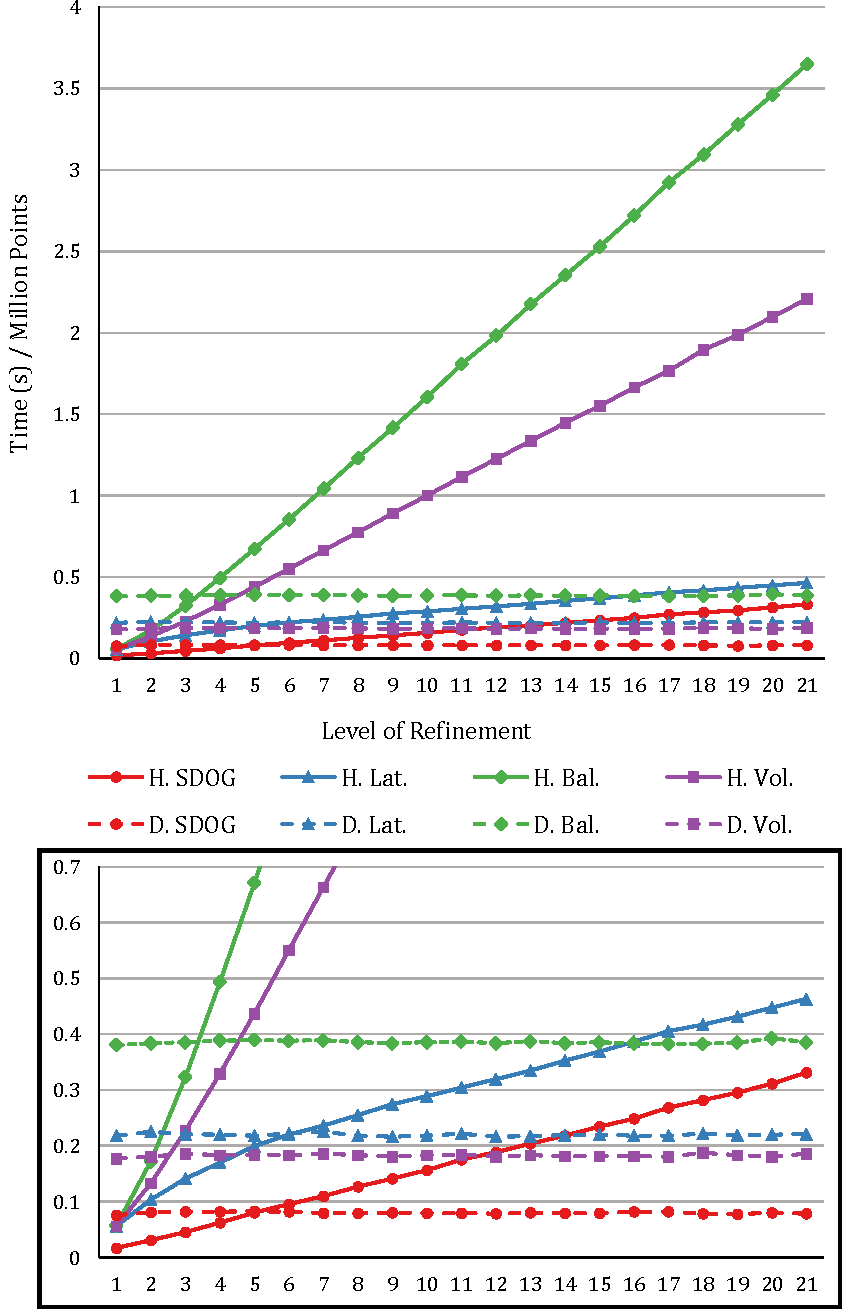
\includegraphics[width=0.8\textwidth]{point-to-index.pdf}
	\caption[Runtime comparison of SDOG point encoding algorithms]{
		A caption will go here.
		The caption may be long.
		This is text that is filling space so that this placeholder caption is longer than if the text was not here.
		Caption caption caption.
		Now the text will repeat...
		A caption will go here.
		The caption may be long.
	}
	\label{fig:point-to-index}
\end{figure}


\subsection{Decoding Algorithm}
\subsubsection{Runtime Comparison}


\begin{figure}[htp!]
	\centering
	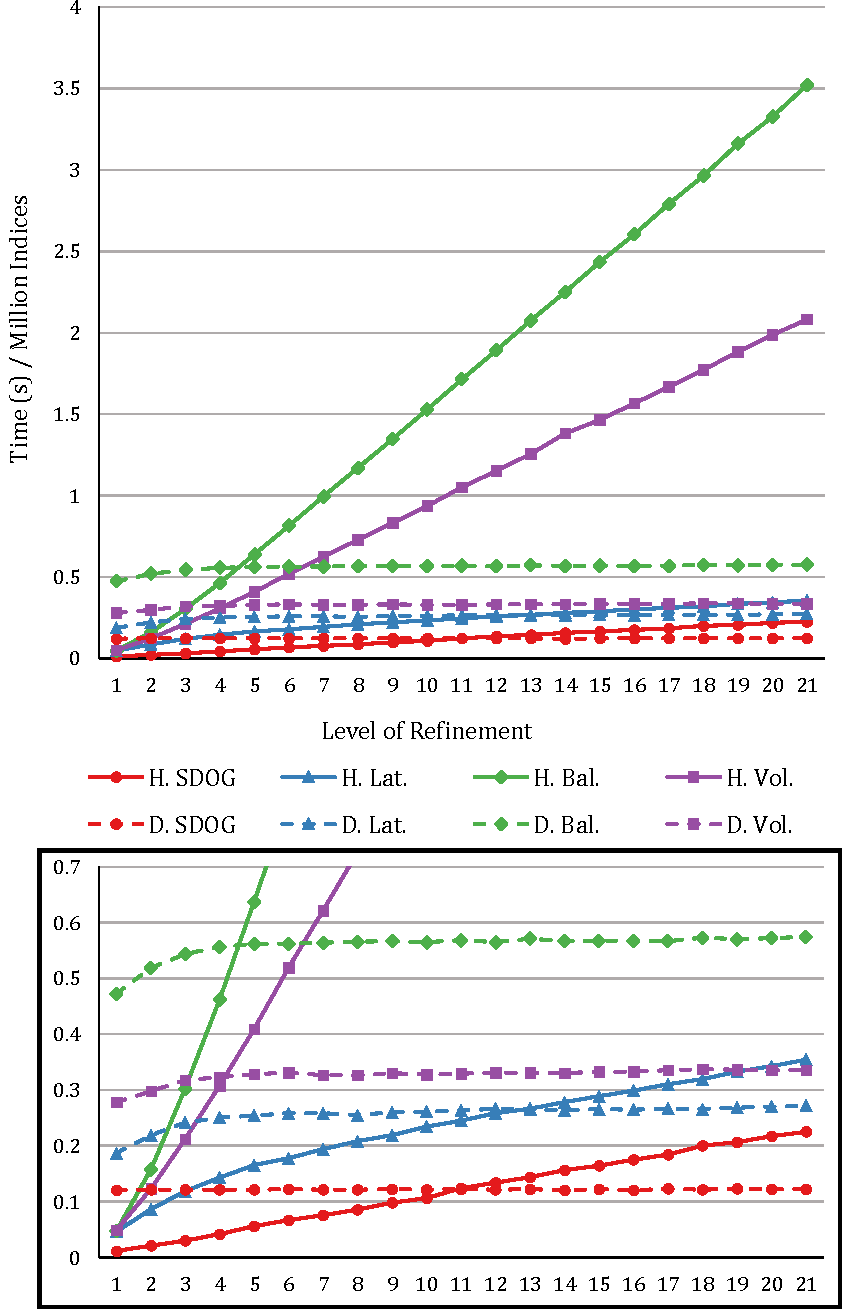
\includegraphics[width=0.8\textwidth]{index-to-range.pdf}
	\caption[Runtime comparison of SDOG decoding algorithms]{
		A caption will go here.
		The caption may be long.
		This is text that is filling space so that this placeholder caption is longer than if the text was not here.
		Caption caption caption.
		Now the text will repeat...
		A caption will go here.
		The caption may be long.
	}
	\label{fig:index-to-range}
\end{figure}
\subsection{Indexing Operations}


\section{Extension Method}
\subsection{Encoding Algorithm}
\subsection{Decoding Algorithm}
\subsection{Indexing Operations} \label{sec:indexing}
An important component of a conventional DGGS is the indexing scheme for cells.
Indices in a DGGS are used to not only identify and linearize cells but also as a means of navigating the grid for various spatial queries~\cite{alderson2020digital}.
To this end, it is important to be able to perform certain operations on said indices efficiently.
The most fundamental of these operations are parent queries, which return the parent (or with non-congruent refinement, \textit{parents}) of a given cell; child queries, which return the children of the cell; and neighbour queries, which return cells that share an edge (or in 3D a face) with the cell.
These operations serve as the building blocks for more complex geospatial queries done with the grid system, such as region growing, data convolution and correlation, feature rasterization, and buffering.
Because of this, creating suitable indexing for a 3D DGGS is an essential task.


With our method---similar to encoding and decoding---we define these operations in terms of surface and radial components.
This split not only simplifies the problem of indexing but also ensures the 3D indexing is consistent with that of the input DGGS.
Referring back to Figures~\ref{fig:indexing} and \ref{fig:3d-coding}, we let $i_s$ be the surface index of a cell and $i_\ell$ be the layer index.
For each of these components, we assume there is a corresponding parent, child, and neighbour operation.
For the surface index, this comes directly from the input DGGS indexing, whereas for the layer index, these would need to be defined.
Using the component operations, we define the corresponding 3D operations as follows.


\paragraph{Parents}
The parent(s) of a cell depend on if the layer of the cell and its parent layer have the same, or different, values of $k_s$.
Let $i_\ell' = \operatorname{parent}(i_\ell)$; if the value of $k_s$ is the same, then the single parent is simply $(i_s, i_\ell')$.
In most cases, the value of $k_s$ for $i_\ell'$ is some number $m$ (often one, but not always) less than that of $i_\ell$.
In this case, the parent(s) are given by $\operatorname{parents}^m(i_s) \times i_\ell$.


\paragraph{Children} The children of a cell depend on if the cell belongs to a central or normal layer.
For normal layers, the set of children is simply $\operatorname{children}(i_s) \times \operatorname{children}(i_\ell)$.
For central layers, the child who belongs to the new central layer must be distinguished from the other child layer(s).
Call the index of the new central layer $c_\ell$; then, this child is given by $(i_s, c_\ell)$.
Let $ N_\ell$ give the set of the other children layer indices (normal layers).
These layers have the surface refinement applied $w$ times, so the resulting children are $\operatorname{children}^w(i_s) \times N_\ell$


\paragraph{Neighbours} We split neighbours into three categories: neighbours in the same layers as the cell, neighbours in the layer above the cell, and neighbours in the layer below the cell.
If a cell belongs to the outermost or innermost (central) layer, then it will not have neighbours in the layer above or below, respectively.
Neighbours in the same layer are simply $\operatorname{neighbours}(i_s) \times i_\ell$.
Let $i_\ell^+$ be the layer above $i_\ell$ and $i_\ell^-$ be the layer below.
If $i_\ell^+$ has the same value of $k_s$ as $i_\ell$, then the single neighbour above is $(i_s, i_\ell^+)$.
In the other case, where the value of $k_s$ for $i_\ell^+$ is some number $m$ greater than that of $i_\ell$, the neighbours are given by $\operatorname{children}^m(i_s) \times i_\ell^+$.
Likewise, if $i_\ell^-$ has the same value of $k_s$ as $i_\ell$, there is one neighbour below given by $(i_s, i_\ell^-)$.
In the case that the value of $k_s$ for $i_\ell^-$ is some number $m$ less than that of $i_\ell$, the neighbours are given by $\operatorname{parents}^m(i_s) \times i_\ell^-$

\section{Summary}